\documentclass[12pt,draftcls,onecolumn]{IEEEtran}
%\documentclass[12pt,onecolumn]{IEEEtran}
\usepackage{times}
\usepackage{hyperref}
%!TEX root =  autocontgrlp.tex
\usepackage{etex}
\usepackage{multicol}
\setlength{\marginparwidth}{13mm}
\usepackage[textsize=tiny]{todonotes}
%\usepackage[disable]{todonotes}
\newcommand{\todoc}[2][]{\todo[color=red!20!white,#1]{Cs: #2}}
\newcommand{\todoch}[2][]{\todo[color=blue!20!white,#1]{C: #2}}
\newcommand{\todos}[2][]{\todo[inline,color=blue!20!white,#1]{S: #2}}
%\usepackage{enumitem}
\usepackage[fleqn]{amsmath}
\usepackage{mathtools}
\usepackage{graphicx}
\usepackage{times}
\usepackage{helvet}
\usepackage{courier}
\usepackage{paralist}
\usepackage{latexsym}
\usepackage{url}
\usepackage[all]{xy}
\usepackage{amsmath}
\usepackage{amssymb}
\usepackage{amsthm}
\usepackage{nccmath} % mfrac
\usepackage{comment}
%\usepackage{enumitem}
\usepackage{paralist}
\usepackage{xcolor}
\usepackage[colorlinks=true,linkcolor=blue,citecolor=purple]{hyperref}
%\usepackage{hyperref}
\usepackage{graphicx}
\usepackage{pifont}
%\usepackage{algorithm}
%\usepackage{algorithmic}
%\usepackage{pseudocode}
%\usepackage{algpseudocode}
\usepackage{savesym}
\savesymbol{AND}
\usepackage{xspace}
\usepackage{tikz}
\usepackage{pgfplots}
\usepackage{pgf}
\usepackage{algorithm}
\usepackage{algorithmic}
\usepackage{xspace}
\usepackage{comment}
\usepackage{placeins}
\usepackage[capitalize]{cleveref}


%\usepackage{style/ssltr}
%\usepackage{style/macros}
\if0
\usetikzlibrary{intersections}
\usetikzlibrary{arrows,calc,fit,patterns,plotmarks,shapes.geometric,shapes.misc,shapes.symbols,   shapes.arrows,   shapes.callouts,   shapes.multipart,   shapes.gates.logic.US,   shapes.gates.logic.IEC,   er,   automata,   backgrounds,   chains,   topaths,   trees,   petri,   mindmap,   matrix,   calendar,   folding, fadings,   through,   positioning,   scopes,   decorations.fractals,   decorations.shapes,   decorations.text,   decorations.pathmorphing,   decorations.pathreplacing,   decorations.footprints,   decorations.markings, shadows,circuits}
\tikzstyle{decision}=[diamond,draw]
\tikzstyle{line}=[draw]
\tikzstyle{elli}=[draw,ellipse]
\tikzstyle{arrow} = [thick]
\fi
%\usepackage{subfig}
\newcommand{\ralp}{r_{\text{ALP}}}
\newcommand{\Jalp}{J_{\text{ALP}}}
\newcommand{\alp}{\text{ALP}\xspace}
\newcommand{\lralp}{\text{RLALP}\xspace}
\newcommand{\mb}{\mbox{ }}
\newcommand{\one}{\mathbf{1}}
\newcommand{\zero}{\mathbf{0}}
\newcommand{\nn}{\nonumber}
\newcommand{\minp}{(\min,+)}
\newcommand{\R}{\mathbf{R}}
\newcommand{\Rm}{\mathbf{R}_{\min}}
\newcommand{\ra}{\rightarrow}
\newcommand{\om}{\otimes}
\newcommand{\op}{\oplus}
\newcommand{\RA}{\Rightarrow}
\newcommand{\LA}{\Leftarrow}
\newcommand{\E}{\mathbf{E}}
\newcommand{\T}{\mathcal{T}}
\newcommand{\B}{\mathcal{B}}
\newcommand{\F}{\mathcal{F}}
\newcommand{\C}{\mathcal{C}}
\newcommand{\M}{\mathcal{M}}
\newcommand{\N}{\mathcal{N}}
\newcommand{\et}{||\Gamma J^*-\hg J^*||_\infty}
\newcommand{\etmn}{||\Gamma J^*-\hg J^*||_{\mn}}
\newcommand{\ini}{\lceil \frac{n}{k}\rceil}
\newcommand{\I}{\mathcal{I}}
\newcommand{\mut}{\tilde{\mu}}
\newcommand{\mn}{\infty,\psi}
\newcommand{\tj}{\tilde{J}}
\newcommand{\hj}{\hat{J}}
\newcommand{\jd}{J'}
\newcommand{\bj}{\bar{J}}
\newcommand{\tv}{\tilde{V}}
\newcommand{\hv}{\hat{V}}

\newcommand{\tu}{\tilde{u}}
\newcommand{\hu}{\hat{u}}

\newcommand{\muh}{\hat{\mu}}
\newcommand{\mui}{{\mu}^i}

\newcommand{\br}{\bar{r}}
\newcommand{\hr}{\hat{r}}
\newcommand{\har}{\hat{r}}
\newcommand{\tr}{\tilde{r}}
\DeclareMathOperator{\argmin}{argmin}
\DeclareMathOperator{\argmax}{argmax}
\newcommand{\norm}[1]{\|#1\|}
\newcommand{\inorm}[1]{\|#1\|_{\infty}}
\newcommand{\snorm}[1]{\left\|#1\right\|}
\newcommand{\sinorm}[1]{\left\|#1\right\|_{\infty}}


%\newcommand{\eqdef}{\stackrel{\text{\footnotesize def}}{=}}
%\newcommand{\eqdef}{\stackrel{\Delta}{=}}
\newcommand{\eqdef}{\doteq}
\newcommand{\defeq}{\doteq}

\newcommand{\eps}{\varepsilon}
\renewcommand{\epsilon}{\varepsilon}



\newcommand{\tg}{\tilde{\Gamma}}



\newcommand{\conf}{\sqrt{\frac{2\ln t}{t_i}}}
%\newcommand{\tg}{\tilde{\Gamma}}
\newcommand{\hg}{\hat{\Gamma}}
%\newcommand{\hg}{{\Gamma}_W}
\newcommand{\gd}{\Gamma'}
\newcommand{\vd}{V'}
%\newcommand{\qed}{\blacksquare}

\newcommand{\keywords}[1]{{\bf Keywords: } #1\par}
%\newenvironment{proof}{{\bf Proof:} }{}
\newtheorem{theorem}{Theorem}[section]
\newtheorem{lemma}[theorem]{Lemma}
\newtheorem{proposition}[theorem]{Proposition}
\newtheorem{corollary}[theorem]{Corollary}
\newtheorem{assumption}{Assumption}[section]
\newtheorem{definition}{Definition}[section]
\newtheorem{remark}{Remark}[section]
\newtheorem{example}{Example}[section]
\newtheorem{note}{Note}[section]
\newcommand{\alert}[1]{\textcolor{red}{#1}} 
\newcommand{\J}{\mathcal{J}}


\def\v{\mathbf{v}}
\def\r{\mathbf{r}}
\def\p{\mathbf{p}}
\def\q{\mathbf{q}}
\def\R{\mathrm{R}}
\def\Re{\mathbb{R}}
\def\Z{\mathbb{Z}}
\def\P{\mathrm{P}}
\def\S{\mathcal{S}}
\def\A{\mathcal{A}}

\newcommand{\ith}[2][th]{$#2^{\text{#1}}$}
\newcommand{\us}[2]{\underset{#2}{#1}~}
\newcounter{subequation}[equation]
\newcommand{\thesubequationonly}{\alph{subequation}}
\renewcommand{\thesubequation}{\text{\theequation(\thesubequationonly)}}
\newcommand{\subequationitem}{\refstepcounter{subequation}(\thesubequationonly)\thinspace}

\def\mathdisplay#1{%
  \ifmmode \@badmath
  \else
    $$\def\@currenvir{#1}%
    \let\dspbrk@context\z@
    \let\tag\tag@in@display \SK@equationtrue %\let\label\label@in@display
    \global\let\df@label\@empty \global\let\df@tag\@empty
    \global\tag@false
    \let\mathdisplay@push\mathdisplay@@push
    \let\mathdisplay@pop\mathdisplay@@pop
    \if@fleqn
      \edef\restore@hfuzz{\hfuzz\the\hfuzz\relax}%
      \hfuzz\maxdimen
      \setbox\z@\hbox to\displaywidth\bgroup
        \let\split@warning\relax \restore@hfuzz
        \everymath\@emptytoks \m@th $\displaystyle
    \fi
%   \fi
}

\newcommand{\algorithmicinput}{\textbf{Input:} }
\newcommand{\INPUT}{\item[\algorithmicinput]}
\newcommand{\algorithmicoutput}{\textbf{Output:} }
\newcommand{\OUTPUT}{\item[\algorithmicoutput]}
\newcounter{algostep}
\newcommand{\Step}[1][\STATE]{#1\textbf{\refstepcounter{algostep}\thealgostep}. }

\newenvironment{algoequation}{\refstepcounter{equation}$}{$\hfill (\theequation)}

\newenvironment{nonfloatalgorithm}[1]{\vspace{1ex}\hrule\vspace{0.5ex} \refstepcounter{algorithm}\textbf{Algorithm \thealgorithm}\hspace{1em} #1 \vspace{0.5ex}\hrule}{\hrule\vspace{1.5ex}\setcounter{algostep}{0}}

\newcounter{acalgorithm}

\newenvironment{nonfloatactorcriticalgorithm}[1]{\vspace{1ex}\hrule\vspace{0.5ex} \textbf{Actor-Critic Algorithm \refstepcounter{acalgorithm}\theacalgorithm}\hspace{1em} #1 \vspace{0.5ex}\hrule\addcontentsline{loa}{algorithm}{\protect\numberline{\theacalgorithm}{\ignorespaces #1}}}{\hrule\vspace{1.5ex}\setcounter{algostep}{0}}

%\documentstyle[nips14submit_09,times,art10]{article} % For LaTeX 2.09
\title{A Generalized Reduced Linear Program for Markov Decision Processes}
\author{Chandrashekar Lakshminarayanan and Shalabh Bhatnagar\\Department of Computer Science and Automation\\ Indian Institute of Science\\ Bangalore-560012\\\{chandrul,shalabh\}@csa.iisc.ernet.in\\ and \\
Csaba Szepesv\'{a}ri\\Department of Computing Science\\University of Alberta\\Edmonton, Alberta\\Canada T6G 2E8\\  szepesva@cs.ualberta.csa }


% The \author macro works with any number of authors. There are two commands
% used to separate the names and addresses of multiple authors: \And and \AND.
%
% Using \And between authors leaves it to \LaTeX{} to determine where to break
% the lines. Using \AND forces a linebreak at that point. So, if \LaTeX{}
% puts 3 of 4 authors names on the first line, and the last on the second
% line, try using \AND instead of \And before the third author name.
\newcommand{\fix}{\marginpar{FIX}}
\newcommand{\new}{\marginpar{NEW}}
%\nipsfinalcopy % Uncomment for camera-ready version
\begin{document}
\maketitle
\begin{abstract}
The term Approximate Dynamic Programming (ADP) refers to a gamut of approximate solution methods for MDPs with large number of states. Though various ADP algorithms are known till date, very few of them successfully address both the prediction and the control problems. Approximate Linear Programming (ALP) is an ADP method that offers sound theoretical guarantees and solves both the prediction and the control problems. Nevertheless, ALP has a serious limitation in that it has large number of constraints, and in practice, a reduced linear program (RLP) is solved instead. Though the RLP has been shown to perform well empirically, error bounds are available only for a specific RLP obtained under idealized assumptions.\\
In this paper, we generalize the RLP to define a generalized reduced linear program (GRLP) which has a tractable number of constraints that are obtained as positive linear combinations of the original constraints of the ALP. The main contribution of this paper is the novel theoretical framework developed to obtain error bounds for any given GRLP. Central to our framework are two $\max$-norm contraction operators. Our result also theoretically justifies linear approximation of constraints. We discuss the implication of our results in the contexts of ADP and reinforcement learning.
\end{abstract}
\begin{keywords}{
Approximate Dynamic Programming (ADP), Markov Decision Processes (MDPs), Approximate Linear Programming (ALP), Generalized Reduced Linear Program (GRLP), Constraint Sampling, Reinforcement Learning.}
\end{keywords}


\section{Introduction}\label{intro}
Optimal sequential decision making problems occurring in science, engineering and economics can be cast in the framework of Markov Decision Processes (MDPs). A policy $u$, is a mapping from state space to action space and it specifies the action selection mechanism. The problem of \emph{control} requires coming up with good policies and for which one needs to \emph{predict} the behavior of individual policies. The problem of \emph{prediction} deals with computing the value-function $J_u$\footnote{Also known as reward/cost-to-go function.} (a mapping from state space to reals) which specifies the value of each state under a given policy $u$. In order to solve an MDP it is necessary to solve the problem of prediction as well as the problem of control.\\
Given an MDP, ideally, we would be interested in computing the optimal value function $J^*$ and the optimal policy $u^*$. The Bellman equation (BE) relates these quantities. Conventional solution methods for MDPs \cite{BertB} such as value iteration, policy iteration and linear programming can compute exact values of $J^*$ and $u^*$ by either directly or indirectly solving the Bellman equation. By computing $J^*$ and $u^*$, the conventional methods address both the prediction and control problems. However, due to the curse-of-dimensionality, the size of the state space grows exponentially in the number of state variables and as a consequence most MDPs arising from practical applications have a large number of states. It is hence difficult to compute the exact values of $u^*$ and $J^*$ for MDPs with large number of states and the usage of conventional methods to solving MDPs is limited.\\
Approximate Dynamic Programming (ADP) \cite{dpchapter,powell} refers to a gamut of approximate solution methods to MDPs with large number of states. In order to reduce the computational effort, ADP methods resort to dimensionality reduction by parameterizing the value function and/or the policy and restricting their search space to the chosen parameterized class. Thus, instead of computing exact values of $u^*$ and $J^*$, ADP methods only compute an approximate value function $\tilde{J}$ and a sub-optimal policy $\tilde{u}$. The quality of the ADP method is measured by the error $||J^*-\tilde{J}||$, in approximating the value function and the loss in performance due to the sub-optimal policy $||J^*-J_{\tilde{u}}||$, measured with respect to the optimal policy. Of the two error terms, $||J^*-J_{\tu}||$ is more important because ultimately we are interested in the problem of finding a useful policy. In the context of ADP, the prediction and control problems are said to be addressed when the errors $||J^*-\tilde{J}||$ and $||J^*-J_{\tilde{u}}||$ can be bounded so that the loss in performance due to the approximation can be quantified.\\
Value-function-only\footnote{Since this paper is concerned with results related to the Approximate Linear Programming formulation we do not discuss other classes of ADP methods such as \emph{actor-only} and \emph{actor-critic} methods.} (or \emph{critic-only}) ADP methods approximate the value function and use it to obtain a one-step look ahead policy by making use of the Bellman equation. Most widely used parameterization to approximate the value function is the linear function approximator (LFA). Methods employing LFA approximate the value function as $J_u\approx\Phi r^*$, where $\Phi$ is a feature matrix whose columns are the basis functions and $r^*$ is a weight vector to be learnt. Dimensionality reduction is achieved by choosing fewer number of basis functions compared to the number of states.\\
A host of value-function-based ADP methods solve the Projected Bellman equation (PBE) which is obtained by including the least squares projection operator in the BE so as to project quantities onto the lower dimensional subspace. A limitation of using the least squares projection operator is that it reduces the prediction error $L_2$-norm and cannot ensure policy improvement which requires prediction error to be minimum in the $L_\infty$-norm. Due to this norm mismatch, policy improvement cannot be guaranteed and \emph{policy-chattering} (policy-oscillations) can occur in practice \cite{dpchapter}. Thus the fundamental issue with the PBE based methods is that they fail to address the control problem.\\
The approximate linear programming (ALP) \cite{ALP,CS,SALP,ALP-Bor,gkp,fs,npalp} formulation also employs LFA, however, solves a linear program to compute $J^*\approx\tilde{J}=\Phi r^*$, and computes a one-step greedy policy. Since the ALP computes an approximation to $J^*$ and outputs only a single policy $\tilde{u}$, there is no issue of \emph{policy-chattering}. The ALP formulation also provides theoretical performance guarantees, i.e., both error terms $||J^*-\tilde{J}||$ and $||J^*-J_{\tilde{u}}||$ can be bounded. This makes the ALP an attractive method since it addresses both the prediction and control problems. However, an important shortcoming of the ALP is that the number of constraints are of the order of the state space. Due to the curse, the number of constraints can be large for practical MDPs and is a limitation.\\
In practice, the issue of large number of constraints in the ALP has been tackled by a procedure known as constraint sampling, wherein a subset of the original constraints of the ALP are sampled to formulate a reduced linear program (RLP). The RLP has been shown to perform well in experiments \cite{ALP,CS,CST} in various domains such as Tetris and in network of queues. However, the theoretical results \cite{CS} are available only for a specific RLP formulated under idealized conditions. Thus, there is a gap in the theoretical understanding of RLP and constraint reduction/approximation. Our aim in this paper is to provide theoretical guarantees which will make the RLP a complete ADP method that addresses both the prediction and the control problems.\\
In this paper, we develop a novel theoretical framework to study a generalized constraint reduction technique namely generalized reduced linear program (GRLP) and present its error analysis. The salient aspects of our contribution are listed below:
\begin{enumerate}
\item \textbf{Framework:}\\ We generalize the RLP to define the GRLP. The GRLP has a small number of constraints which are obtained as positive linear combinations of the original constraints of the ALP. The GRLP serves as a framework to analyze error due to constraint reduction and linear constraint approximation.
\item \textbf{Error Analysis:}
	\begin{itemize}
		\item We develop novel analytical machinery to relate $\hat{J}$, the solution to the GRLP, and the optimal value function $J^*$. 
		\item We show that $||J^*-\hat{J}||\leq (c_1+c_2)$, where $c_1>0$, $c_2>0$ are constants. While the term $c_1$ is error inherent to the ALP formulation itself, the term $c_2$ is the additional error introduced due to constraint approximation.  
		\item We derive a greedy policy $\hu$ by making use of $\hj$ and bound the term $||J^*-J_{\hu}||$. 
		\item Akin to the error analysis in \cite{ALP,CS,SALP} our bounds are also in terms of a modified $L_\infty$-norm.
		\item Our analysis is based on two novel $\max$-norm contraction operators called the least upper bound (LUB) projection operator and the approximate least upper bound projection operator (ALUB). This is another significant difference in comparison to the results on constraint sampling in \cite{SALP,CS} that make use of concentration bounds and hold only with \emph{high} probability.
\end{itemize}
\item \textbf{Significant Results:}
	\begin{itemize}
		\item We provide error bounds for both prediction and control errors, i.e., bound the terms $||J^*-\hj||$ and $||J^*-J_{\hu}||$ in a modified $L_\infty$-norm. Thus, the GRLP is a complete ADP method with performance guarantees for both the prediction as well as control problems. The modified $L_\infty$-norm allows us to choose the quality of approximation across various states. This makes our result an important addition to the theory of ALP \cite{ALP,CS,CST,SALP}.
		\item The structure of the error terms also reveals an important result that it is not always necessary to sample using the stationary distribution of the optimal policy. This throws additional light on constraint sampling by providing a better explanation for its empirical success even in those cases when sampling distributions other than the stationary distribution of the optimal policy was used. 
		\item Our results on the GRLP are the first to theoretically justify linear function approximation of the constraints. This means that constraint reduction is not only limited to sampling but also can be extended to include linear combinations of constraints.
	\end{itemize}
\item We also discuss the implication of our results in the context of reinforcement learning and also present a numerical example illustrating the theory developed. A short and preliminary version of this paper without the theoretical analysis is available in \cite{aaaipaper}.
\end{enumerate}


\section{Markov Decision Processes (MDPs)}
In this section, we briefly discuss the basics of Markov Decision Processes (MDPs) (the reader is referred to \cite{BertB,Puter} for a detailed treatment).\\
An MDP is a $4$-tuple $<S,A,P,g>$, where $S$ is the state space, $A$ is the action space, $P$ is the probability transition kernel and $g$ is the reward function. We consider MDPs with large but finite number of states, i.e., $S=\{1,2,\ldots,n\}$ for some large $n$, and the action set is given by $A=\{1,2,\ldots,d\}$. For simplicity, we assume that all actions are feasible in all states. The probability transition kernel $P$ specifies the probability $p_a(s,s')$ of transitioning from state $s$ to state $s'$ under the action $a$. We denote the reward obtained for performing action $a\in A$ in state $s\in S$ by $g_a(s)$.\\
A policy $\mu$ specifies the action selection mechanism, and is described by the sequence $\mu=\{u_1,u_2,\ldots,u_n,\ldots\}$, where $u_n\colon S \ra A, \mbox{ }\forall n \geq 0$. A stationary deterministic policy (SDP) is one where $u_n\equiv u, \mbox{ }\forall n\geq 0$ for some $u\colon S \ra A$. By abuse of notation we denote the SDP by $u$ itself instead of $\mu$. In the setting that we consider, one can find an SDP that is optimal \cite{BertB,Puter}. In this paper, we restrict our focus to the class $U$ of SDPs.  Under an SDP $u$, the MDP is a Markov chain with probability transition kernel $P_u$.\\
Given an SDP $u$, the infinite horizon discounted reward corresponding to state $s$ under $u$ is denoted by $J_u(s)$ and is defined by
\begin{align}
J_u(s)\stackrel{\Delta}{=}\E[\sum_{n=0}^\infty \alpha^n g_{a_n}(s_n)|s_0=s,a_n=u(s_n)\mbox{ }\forall n\geq 0],\nn
\end{align}
where $\alpha \in (0,1)$ is a given discount factor. Here $J_u(s)$ is known as the value of the state $s$ under the SDP $u$, and the vector quantity $J_u\stackrel{\Delta}{=}(J_u(s), \forall s\in S)^\top\in R^n$ is called the value-function corresponding to the SDP $u$.\\
The optimal policy $u^*$ is obtained as $u^*(s)\stackrel{\Delta}{=}\arg\max_{u\in U}J_u(s)$\footnote{Such $u^*$ exists and is well defined in the case of infinite horizon discounted reward MDP, for more details see \cite{Puter}.}. The optimal value-function $J^*$ is the one obtained under the optimal policy, i.e., $J^*=J_{u^*}$. Given an MDP, our aim is to find the optimal value function $J^*$ and the optimal policy $u^*$. The optimal policy and value function obey the Bellman equation (BE) as under: $\forall s \in S$,
\begin{subequations}\label{bell}
\begin{align}
\label{bellval}J^*(s)&=\max_{ a\in A}\big(g_a(s)+\alpha \sum_{s'}p_a(s,s')J^*(s')\big),\\
\label{bellpol}u^*(s)&=\arg\max_{ a\in A}\big(g_a(s)+\alpha \sum_{s'}p_a(s,s')J^*(s')\big).
\end{align}
\end{subequations}
Typically $J^*$ is computed first and $u^*$ is obtained by substituting $J^*$ in \eqref{bellpol}. The Bellman operator $T$ is defined using the model parameters of the MDP as follows:
\begin{definition}
\begin{align}
(TJ)(s)=\max_{a \in A}\big(g_a(s)+\alpha \sum_{s'} p_a(s,s')J(s')\big), 
\end{align}
where $J\in \R^n$. Similarly one can define the Bellman operator restricted to an SDP $u$ as follows:
\begin{align}
(T_uJ)(s)=\big(g_{u(s)}(s)+\alpha \sum_{s'} p_{u(s)}(s,s')J(s')\big).
\end{align}
\end{definition}
Given $J \in \R^n$, $TJ$ is the `one-step' greedy value function. It is also useful to define the notion of a one-step greedy policy as below:
\begin{definition}
A policy $\tilde{u}$ is said to be greedy with respect to $\tilde{J}$ if
\begin{align}\label{subpol}
\tilde{u}(s)=\underset{a \in A}{\arg\max}(g_a(s)+\alpha\sum_{s'} p_a(s,s')\tilde{J}(s')).
\end{align}
\end{definition}
\begin{definition}
We also define the $Q$-Bellman operator \cite{BertB} $H$. Given any $J\in \R^n$ we have,

\begin{align}
HJ&=\left[ {\begin{array}{c} H_1 J  \\ \vdots \\ H_d J\end{array}} \right]\in \R^{nd},\mbox{where}\nn\\
(H_a J)(s)&= g_a(s)+\alpha \sum_{s'}p_a(s,s') J(s'), \forall s\in S, a\in A,
\end{align}
\end{definition}
 We now state without proof the important properties related to the Bellman operator. Though in these results, we make use of the Bellman operator $T$, the results also trivially hold for $T_u$ as well.
\subsection{Properties of $T$}
\begin{lemma}\label{maxnorm}
$T$ is a $\max$-norm contraction operator, i.e., given $J_1, J_2 \in \mathbf{R}^n$,
\begin{align}
||TJ_1-TJ_2||_\infty\leq \alpha ||J_1-J_2||_\infty.
\end{align}
\end{lemma}
\begin{corollary}\label{uniquesol}
$J^*$ is a unique fixed point of $T$, i.e., $J^*=TJ^*$.
\end{corollary}
The Bellman operator $T$ exhibits two more important properties presented in the following lemmas (see \cite{BertB} for proofs):
\begin{lemma}\label{monotone}
$T$ is a monotone map, i.e., given $J_1,J_2 \in \R^n$ such that $J_2\geq J_1$, we have $T J_2\geq T J_1$. Further, if $J\in \R^n$ is such that $J\geq TJ$, it follows that $J\geq J^*$.
\end{lemma}
\begin{lemma}\label{shift}
Given $J\in \R^n$, $t \in \R$ and $\mathbf{1} \in \R^n$, a vector with all entries $1$, we have
\begin{align}
T(J+t\mathbf{1})=TJ+\alpha t\mathbf{1}.
\end{align}
\end{lemma}
Note that Lemmas~\ref{maxnorm}-\ref{shift} also hold for the $Q$-Bellman operator $H$.
Solving an MDP involves handling two sub-problems namely the problem of \emph{control} and the problem of \emph{prediction}. The problem of \emph{control} deals with coming up with a good (and if possible the optimal) policy. Often, in order to solve the problem of \emph{control}, one needs to solve the problem of \emph{prediction}, which deals with computing the value function $J_u$ of the policy $u$. The fact that the two problems are related is reflected in the Bellman equation in \eqref{bell}, where $J^*$ from \eqref{bellval} is used in \eqref{bellpol} to obtain the optimal policy $u^*$. Thus, the Bellman equation is at the heart of the solution methods to MDPs. Any solution method to MDP is said to be complete only if it satisfactorily (with provable performance guarantees) addresses both the prediction and the control problems. \\
The basic solution methods namely value iteration, policy iteration and linear programming (LP) formulation \cite{BertB} solve both the control and prediction problems. Of the three basic methods, in this paper, we are interested in the LP formulation given by
\small
\begin{align}\label{mdplp}
\min_{J\in \R^n} &c^\top J\nn\\
\text{s.t}\mb &J(s)\geq g_a(s)+\alpha\sum_{s'}p_a(s,s')J(s'), \mb\forall s\in S, a \in A,
\end{align}
\normalsize
where $c\in \R^n_+$ is any vector whose components are all non-negative. One can show that $J^*$ is the solution to the LP formulation \eqref{mdplp} \cite{BertB}. 
Also, of the three methods, value iteration and LP formulation are value function based methods, i.e., they compute $J^*$ directly and then $u^*$ is obtained by plugging $J^*$ in \eqref{bellpol}.\\
While the basic methods (i.e., VI, PI and LP) can be used to compute exact values $J^*$ and $u^*$ for MDPs with a small number of states, they are computationally expensive in the case of MDPs with a large number of states.
\section{Approximate Dynamic Programming}
\emph{Curse-of-Dimensionality} is a term used to denote the fact that the number of states grows exponentially in the number of state variables. Most MDPs arising in practical applications suffer from the curse, i.e., have large number of states and it is difficult to compute $J^*/J_u\in \R^n$ exactly in such scenarios. Approximate dynamic programming (ADP) \cite{lspi,lspe,ALP,wang2014approximate} methods compute an approximate value function $\tilde{J}$ instead of $J^*/J_u$. In order to tackle the curse, ADP methods resort to dimensionality reduction by parameterizing the value function and/or the policy. Value-function based ADP methods form an important subclass of ADP methods whose brief overview is given below.
\subsection{Value-Function based ADP}
In the value-function based ADP schemes a parameterized family is chosen and the approximate value-function $\tilde{J}$ is picked from the chosen parameterized class.
Once the approximate value function $\tilde{J}$ is computed, a sub-optimal policy $\tilde{u}$ can be obtained as the one-step greedy policy with respect to $\tilde{J}$ by making use of \eqref{subpol}.
The following lemma characterizes the degree of sub-optimality of the greedy policy $\tilde{u}$.
\begin{lemma}\label{subopt}
Let $\tilde{J}$ be the approximate value function and $\tilde{u}$ be as in \eqref{subpol}, then 
\begin{align}
||J^*-J_{\tilde{u}}||_\infty \leq \frac{2}{1-\alpha}||J^*-\tilde{J}||_\infty.
\end{align}
\end{lemma}
The quality of any ADP method depends on the approximation guarantees it offers for the quantities $||J^*-\tilde{J}||$ and $||J^*-J_{\tu}||$, where $||\cdot||$ is an appropriate norm. The term  $||J^*-\tilde{J}||$ denotes the error in prediction and $||J^*-J_{\tu}||$ denotes the loss in performance resulting from the sub-optimal policy $\tu$ with respect to the optimal policy $u^*$. Of the two error terms, $||J^*-J_{\tu}||$ is more important because ultimately we are interested in coming up with a useful policy. In the context of ADP methods, the control and prediction problems are said to be addressed when the error terms $||J^*-\tilde{J}||$ and $||J^*-J_{\tu}||$ are bounded by ``small'' constants.\\
\subsection{Linear Function Approximation}
The most widely used parameterized class to approximate the value-function is the linear function approximator (LFA). Under LFA, the value-function is approximated as $\tilde{J}=\Phi r^*$, with $\Phi=[\phi_1|\ldots|\phi_k]$ being an $n\times k$ feature matrix and $r^*$ is the parameter to be learnt.\\
There are two important approaches to value function approximation. Both the approaches start out with a basic solution method and appropriately introduce function approximation in it. The two approaches are:
\begin{enumerate}
\item The Projected Bellman Equation (PBE) which combines the BE and the linear least squares projection operator to project high dimensional quantities onto the subspace of the LFA.
\item The approximate linear programming formulation which introduces the LFA in the linear programming formulation. 
\end{enumerate}
A host of ADP methods are based on the PBE and have been found to be useful in practice. The main application of the PBE is for approximate policy evaluation, i.e., to compute $\tilde{J}_u$, an approximation to the value function $J_u$ of policy $u$. Due to the mismatch in the norms, i.e, the linear least squares projection operator based on the $L_2$-norm and the $L_\infty$-norm of the Bellman operator $T$, one cannot use the PBE to obtain a direct approximation to $J^*$. Thus in order to solve the problem of control, $\tilde{J}_u$ is used to compute a one-step greedy policy. However, again due to the mismatch in the norms, i.e., $L_2$-norm of the linear least squares projection and the $L_\infty$ norm required for policy improvement (Lemma~\ref{subopt}), the one-step greedy policy need not necessarily be an improvement. This leads to a phenomenon called \emph{policy-chattering} \cite{dpchapter} where looping within of bad policies can occur. Further, such policy-chattering can be demonstrated in simple examples as well \cite{dpchapter}. Thus, though the approximate value function obtained by solving the PBE offers guarantees for prediction it does not offer any guarantees for the control problem, a significant shortcoming of the PBE based methods.\\
The ALP formulation \cite{ALP} on the other hand does not suffer from issues such as policy-chattering, for the simple reason that it computes $\tilde{J}$ which is an approximation to $J^*$ and a one-step greedy policy $\tilde{u}$ obtained using $\tilde{J}$. In short, since there is only one policy that the ALP outputs there is no question of policy-chattering. Further, the ALP offers performance guarantees for both the error terms $||J^*-\tilde{J}||$ and $||J^*-J_{\tilde{u}}||$. Though the ALP is a complete method addressing both the control and prediction problems, it nevertheless suffers from an important limitation in the form of large number of constraints (as large as the size of the state space). This limitation has been addressed in literature by sampling only a fewer tractable constraints to formulate a reduced linear program (RLP). The RLP has been shown to perform well in practice \cite{ALP,CS,CST}, but theoretical performance guarantees \cite{CS} are available for a specific RLP obtained under idealized assumptions. In this paper, by providing a sound theoretical analysis of the RLP, we aim to show that RLP is a complete method that addresses both the prediction and the control problems.
We achieve this by developing and presenting a comprehensive theoretical framework to understand the constraint reduction/approximation procedure.\\
In the next section, we discuss the approximate linear programming (ALP) formulation, the basic results and present prior results in literature as well as motivate the problem that we address in this paper. 

\section{Approximate Linear Programming}
The LP formulation in \eqref{mdplp} can be represented in short as,
\begin{align}\label{mdplpshort}
\min_{J\in \R^n} &c^\top J\nn\\
\text{s.t}\mb &J\geq T J,\\
\textbf{or}\nn\\
\label{shortalter}
\min_{J\in \R^n} &c^\top J\nn\\
\text{s.t}\mb &EJ\geq H J,\\
\end{align}
where $J\geq TJ$ is a shorthand for the $nd$ constraints in \eqref{mdplp} and $E$ is an $nd\times n$ matrix given by $E=[I,\ldots,I]^\top$, i.e., $E$ is obtained by stacking $d$ identical $n\times n$ identity matrices one over the other. Note that \eqref{mdplpshort} and \eqref{shortalter} are identical programs and differ only in notation. We use notation of type \eqref{mdplpshort} whenever we prefer brevity and we use notation \eqref{shortalter} in some definitions and proof for the sake of clarity.
The approximate linear program (ALP) is obtained by making use of LFA in the LP, i.e., by letting $J=\Phi r$ in \eqref{mdplpshort} and is given as
\begin{align}\label{alp}
\min_{r\in \R^k} &c^\top \Phi r\nn\\
\text{s.t}\mb &\Phi r\geq T \Phi r.
\end{align}
Unless specified otherwise we use $\tr$ to denote the solution to the ALP and $\tj=\Phi \tr$ to denote the corresponding approximate value function. We now state the assumptions and definitions used for the rest of the paper.
\begin{assumption}\label{one}
The first column of the feature matrix $\Phi$ (i.e., $\phi_1$) is $\one \in \R^n$. In other words, the constant function is part of the basis.
\end{assumption}
\begin{assumption}\label{probdist}
$c=(c(i),i=1,\ldots,n)\in \R^n$ is a probability distribution, i.e., $c(i)\geq 0$ and $\sum_{i=1}^n c(i)=1$.
\end{assumption}
\begin{definition}
Given a function $\chi\colon S\ra \R^+$ we define the quantity $\beta_{\chi}$ as
\begin{align}
\beta_{\chi}=\max_{s \in S} \frac{\underset{a \in A}{\max}\big(\alpha\sum_{s'}p_a(s,s')\chi(s')\big)}{\chi(s)}.
\end{align}
\end{definition}
\begin{definition}
The function $\chi$ is then said to be a \emph{Lyapunov} function if $\beta_{\chi}<1$.
\end{definition}
\begin{assumption}\label{lyap}
$\psi\colon S \ra \R^+$ is a Lyapunov function and is present in the column span of the feature matrix $\Phi$.
\end{assumption}
It is straightforward to check that the function $\one$ is a Lyapunov function and trivially is present in the column span of $\Phi$. 
\begin{definition}\label{modlone}
The modified $L_1$-norm is defined as
\begin{align}
||J||_{1,c}=\sum_{s \in S} c(s)|J(s)|,
\end{align}
where $c$ obeys Assumption~\ref{probdist}.
\end{definition}
\begin{definition}\label{modnorm}
The modified $L_\infty$-norm is defined as follows:
\begin{align}
||J||_{\infty,\rho}=\max_{s \in S} \rho(s) |J(s)|,
\end{align}
where $\rho \colon \S \ra \R^+$, $J\in \R^n$.
\end{definition}
In Definition~\ref{modnorm}, the use of the weighting function $\rho$ allows us to measure the error taking into account the relative importance of the various states. A lower value of $\rho(s)$ means that the state $s$ is less important and vice-versa.\\
We recall below Theorem~$4.2$ of \cite{ALP} which bounds the error in the approximate value function.
\begin{theorem}\label{restateval}
Let $\tr$ be the solution to the ALP in \eqref{alp}, $\tilde{J}_c=\Phi \tilde{r}_c$, $\psi$ be a Lyapunov function and $c$ be a distribution as in \eqref{probdist}, then 
\begin{align}
||J^*-\tj||_{1,c}\leq \frac{2c^\top \psi}{1-\beta_{\psi}}\min_{r}||J^*-\Phi r||_{\mn}.
\end{align}
\end{theorem}
We now recall Theorem~$3.1$ of \cite{ALP} that characterizes the loss in performance of the greedy policy.
\begin{theorem}\label{restatepol}
Let $\tilde{u}$ be the greedy policy with respect to the solution $\tj$ of the ALP, then 
\begin{align}
||J^*-J_{\tu}||_{1,c}\leq \frac{1}{1-\alpha}||J^*-\tj||_{1,c'},
\end{align}
where $c'=(1-\alpha)c^\top(I-\alpha P_{\tu})^{-1}$.
\end{theorem}
Theorems~\ref{restateval} and ~\ref{restatepol} together imply that the ALP addresses both the control and prediction problems. Please refer to \cite{ALP} for a more detailed treatment of the ALP.\\
Note that the ALP is a linear program in $k$ ($<<n$) variables as opposed to the LP in \eqref{mdplpshort} which has $n$ variables. Nevertheless, the ALP has $nd$ constraints (same as the LP) which is an issue when $n$ is large and calls for constraint approximation/reduction techniques.

\section{Constraint sampling}
The most important work in the direction of constraint reduction is constraint sampling \cite{CS} wherein a reduced linear program (RLP) is solved instead of the ALP. While the objective function of the RLP is the same as that of the ALP, the RLP has only $m<<nd$ constraints sampled from the original ALP according to a given probability distribution. The reduced linear program is then given by
\small
\begin{align}\label{rlp}
\min_{J\in \R^n} &c^\top J\nn\\
\text{s.t}\mb &J(s)\geq g_a(s)+\alpha\sum_{s'}p_a(s,s')J(s'), \mb\forall (s,a) \in \I,
\end{align}
\normalsize
where $\I$ is the index set containing the $m$ sampled state-action pairs. Using the index set $\I$ we define an $nd\times m$ matrix $\M$, called the constraint sampling matrix as below.
\begin{definition}\label{csampmat}
Let $\I=\{(s_1,a_1),\ldots,(s_m,a_m)\}$ be the sampled state-action pairs and let $q_i\stackrel{\Delta}{=}s_i+(a_i-1)\times n,\forall i=1,\ldots,m$. Then the constraint sampling matrix associated with the index set $\I$ is given by
\begin{align}
\M(i,j)&=1, \mb\text{if}\mb q_i=j\nn\\
&=0, \mb\text{otherwise}.
\end{align}
\end{definition}
The RLP can then be represented in short as
\begin{align}\label{rlpshort}
\min_{r\in \N} &c^\top \Phi r\nn\\
\text{s.t}\mb & \M^\top E \Phi r \geq \M^\top H \Phi r,
\end{align}
where $\M$ is a constraint sampling matrix as in Definition~\ref{csampmat} and $\N\subset \R^k$ is a bounded set such that $\tr \in \N$. Note that the feasible set of the RLP is a superset of the feasible set of the ALP.\\
The RLP based on constraint sampling has been found to perform well empirically in application domains ranging from controlled queuing networks (see section $6.2$ of \cite{ALP} and section $7$ of \cite{SALP}) to Tetris (see \cite{CST} and section $6$ of \cite{SALP}). However, the theoretical guarantees for the RLP are available only under a restricted setting \cite{CS}. We present the main result of \cite{CS} on constraint sampling, and to that end define the following:
\begin{definition}\label{sampdist}
Given a policy $u$ and Lyapunov function $\psi$ in the column span of $\Phi$, we define probability distributions $\mu_u$, $\mu_{u,\psi}$ and constant $\theta$ as 
\begin{align}
\mu^\top&\stackrel{\Delta}{=}(1-\alpha)c^\top (I-\alpha P_u)^{-1},\nn\\
\mu_{u,\psi}(s,a)&\stackrel{\Delta}{=}\frac{\mu_{u}(s) \psi(s)}{\mu_u^\top \psi d},\nn\\
\theta&\stackrel{\Delta}{=}\frac{(1+\beta_{\psi})}{2}\frac{\mu_{u^*}^\top \psi}{c^\top J^*}\sup_{r\in \N}||J^*-\Phi r||_{\mn}.
\end{align}
\end{definition}
We now recall Theorem~$3.1$ of \cite{CS} below.
\begin{theorem}\label{csresult}
Let $\epsilon$ and $\delta$ be scalars in $(0,1)$. Let $u^*$ be the optimal policy and $\I$ an index set containing the $m$ state-action pairs sampled independently according to the distribution $\psi_{u^*,\psi}$, for some Lyapunov function $\psi$, where
\begin{align}
m\geq \frac{16d\theta}{(1-\alpha)\epsilon}\big(k\ln\frac{48d\theta}{(1-\alpha)\epsilon}+\ln\frac{2}{\delta}\big).
\end{align}
Let $\tilde{r}$ be an optimal	solution of the ALP and let $\hat{r}$ be the solution of the corresponding RLP, then with probability at least $1-\delta$, we have
\begin{align}
||J^*-\Phi \hat{r}||_{1,c}\leq ||J^*-\Phi \tilde{r}||_{1,c}+\epsilon||J^*||_{1,c}.
\end{align}
\end{theorem}
\textbf{Motivation for our work:}\\
The result in Theorem~\ref{csresult} has a significant limitation in that the sampling distribution $\mu_{u^*,\psi}$ requires the knowledge of $u^*$. The optimal policy $u^*$ might not be available in practice and hence it would not be possible to even formulate the specific RLP for which the bound in Theorem~\ref{csresult} applies. However, as mentioned before, the RLP has performed reasonably well even when the sampling distribution is not $\mu_{u^*,\psi}$. Thus there is a gap between the theoretical understanding of the RLP and its practical efficacy which merits our attention. The gap also indicates that the RLP might be a special case of a generalized constraint reduction scheme with provable performance guarantees. Understanding such a generalized method would result in an ALP based ADP techinque that would have theoretical performance guarantees while being practically useful. In particular, we wish to answer the following open questions.
\begin{itemize}
\item  As a natural generalization of the RLP, what happens if we define a generalized reduced linear program (GRLP) whose constraints are positive linear combinations of the original constraints of the ALP?
\item Unlike \cite{CS} which provides error bounds for a specific RLP formulated using an idealized sampling distribution, is it possible to provide error bounds for any GRLP (and hence any RLP)?
\end{itemize}
In this paper, we address both of the questions above.

\section{Generalized Reduced Linear Program}
In this section we present the generalized reduced linear program (GRLP) which is obtained by appropriately extending the definition of the RLP. An important property that should carry over from the RLP is that the feasible set of the GRLP should also be a superset of the feasible set of the ALP. A natural way to achieve this is to replace the set of sampled constraints in the RLP by a set of constraints which are obtained as linear combinations of the original constraints of the ALP. Formally, we define the generalized reduced linear program (GRLP) as below:
\begin{align}\label{grlp}
\min_{r\in \chi} &c^\top \Phi r,\nn\\
\text{s.t}\mb & W^\top E\Phi r\geq W^\top H \Phi r, 
\end{align}
where $W \in \R_+^{nd\times m}$ is an $nd\times m$ matrix with all nonnegative entries and $\chi \subset \R^k$ is any bounded set such that $\hj \in \chi$. Thus the $i^{th}$ ($1\leq i\leq m$) constraint of the GRLP is a positive linear combination of the original constraints of the ALP. Constraint reduction is achieved by choosing $m<<nd$. The key difference between the RLP in \eqref{rlpshort} and the GRLP in \eqref{grlp} despite their similar structure is that while $\M$ is a matrix of only zeros and ones, $W$ is a matrix of positive entries alone. Also note that an RLP is trivially a GRLP as well. Unless specified otherwise we use $\hr$ to denote the solution to the GRLP in \eqref{grlp}, $\hj=\Phi \hr$, to denote the corresponding approximate value function and $\hu$ to denote the greedy policy with respect to $\hj$.\par
Note that we want to avoid certain uninteresting and trivial cases of $W$ matrix such as $W=0$ or an entire column of $W$ being zero (which means no constraint is generated with respect to that column). Thus it is intuitive to demand that every column of $W$ should be non-negative and have at least one entry which is strictly positive. Also, normalizing columns of $W$ so that they sum to $1$ does not make any difference to the constraints of the RLP. Keeping these in mind we also assume the following throughout the rest of the paper:
\begin{assumption}\label{wassump}
$W \in \R^{nd\times m}_+$ is a full rank $nd\times m$  matrix (where $m<<nd$) and each of its column sums equals $1$.
\end{assumption}
The above assumption is just a technical condition that eliminates uninteresting choices such as $W=0$ or cases when certain columns of $W$ have all zeros, which implies that the corresponding column generates no constraint.

\begin{figure}[h!]
\centering
%\resizebox{columnwidth}{2cm}{
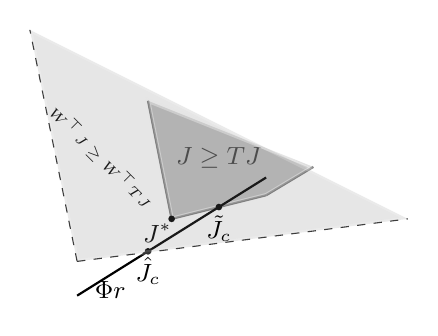
\begin{tikzpicture}[domain=-10:7.7,scale=0.6,font=\small,axis/.style={very thick, ->, >=stealth'}]
%\draw[line,thick,->] (-1,-0.625)--(4,-0.625);
%\draw[line,thick,->] (0,-1)--(0,4);
%\draw[line,thick,-](-0.2,-0.6)--(1,3);
\draw[line,thick,-](0.5,3.5)--(1,1);
\draw[line,thick,-](1,1)--(3,1.5);
\draw[line,thick,-](3,1.5)--(4,2.1);
\node[](one) at (2,2.3){\text{$J\geq TJ$}};
\node[rotate=-45](seven) at (-0.5,2.3){\text{\tiny $W^\top J\geq W^\top TJ$}};
\node[](two) at (-0.3,-0.5){\text{$\Phi r$}};
\node[](three) at (0.7,0.7){\text{$J^*$}};
%\draw[line,thick,-](0,0)--(4,2.5);
 \draw [ultra thick, draw=white, fill=gray, opacity=0.5]
       (0.5,3.5)--(1,1)--(3,1.5)--(4,2.1) -- cycle;
\draw[line,thick,-](-1,-0.625)--(3,1.8750);
 \fill (1,1)  circle[radius=2pt];
 \fill (2,1.25)  circle[radius=2pt];
 \fill (0.5,0.3125)  circle[radius=2pt];
\draw[line,dashed,-](-1,0.1)--(6,1);
\draw[line,dashed,-](-1,0.1)--(-2,5);
 \draw [ultra thick, draw=white, fill=gray, opacity=0.2]
       (-1,0.1)--(6,1)--(-2,5) -- cycle;
\node[] (four) at (2,0.8){\text{$\tilde{J}_c$}};
\node[] (six) at (0.5,-0.1){\text{$\hat{J}_c$}};
\end{tikzpicture}
%}
\caption{The outer lightly shaded region corresponds to GRLP constraints and the inner dark shaded region corresponds to the original constraints. The main contribution of the paper is to bound $||J^*-\hat{J}_c||$.}
\label{cartoon}
\end{figure}


The rest of the paper develops analytically various performance bounds and our main results provide the following:
\begin{enumerate}
\item A bound for $||J^*-\hj||$, the error between the approximate value function $\hj$ as computed by the GRLP and the optimal value function $J^*$;
\item a bound for $||J^*-J_{\hu}||$, the loss in performance due to the greedy policy $\hu$ measured with respect to the optimal policy; and
\item an important result on constraint sampling.
\end{enumerate}
We achieve the above via two novel $\max$-norm contraction operators namely the least upper bound (LUB) projection operator (denoted by $\Gamma$) and the approximate least upper bound (ALUB) projection operator (denoted by $\hat{\Gamma}$). We bound the error due to constraint approximation by analyzing the fixed points of the operators $\Gamma$ and $\hg$. We first establish our results in the $L_\infty$-norm and then extend the same in a modified $L_\infty$-norm. The schematic in Fig. ~\ref{schematic} provides a pictorial representation of what shall follow in the next three sections.
\FloatBarrier
\begin{figure}[h!]
\centering
%\resizebox{columnwidth}{}{
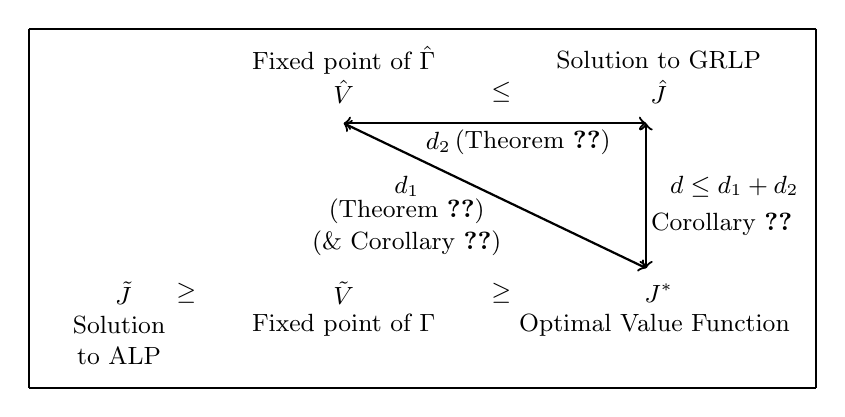
\begin{tikzpicture}[domain=0:7.7,scale=0.8,font=\small,axis/.style={very thick, ->, >=stealth'}]
\draw [line,thick,-] (0,-1)--(0,4.7);
\draw [line,thick,-] (0,4.7)--(12.5,4.7);
\draw [line,thick,-] (12.5,4.7)--(12.5,-1);
\draw [line,thick,-] (0,-1)--(12.5,-1);
\node[](one) at (1.5,0.5) {$\tj$};
\node[](four) at (2.5,0.5) {$\geq$};
\node[](two) at (5,0.5) {$\tv$};
\node[](three) at (10,0.5) {$J^*$};
\node[](five) at (7.5,0.5) {$\geq$};
\node[](six) at (10,3.7) {$\hj$};
\node[](seven) at (5,3.7) {$\hv$};
\node[](eight) at (7.5,3.7) {$\leq$};
\node[](nine) at(1.5,0){\text{Solution }};
\node[](twenty) at(1.5,-0.5	){\text{to ALP }};
\node[](ten) at(5,0){\text{Fixed point of }$\Gamma$};
\node[](eleven) at(10,0){\text{Optimal Value Function }};
\node[](twelve)at (10,4.2){\text{Solution to GRLP}};
\node[](thirteen)at (5,4.2){\text{Fixed point of }$\hg$};
\draw [line,thick,<->] (5,3.2)--(9.8,0.9);
\draw [line,thick,<->] (5,3.2)--(9.8,3.2);
\draw [line,thick,<->] (9.8,3.2)--(9.8,0.9);
\node[](fourteen)at (6,2.2){$d_1$};
\node[](fifteen)at (6.5,2.9){$d_2$};
\node[](sixteen)at (11.2,2.2){$d\leq d_1+d_2$};
\node[](eighteen)at (11,1.6){\text{Corollary~\ref{cmt2}}};
\node[](seventeen)at (8,2.9){\text{(Theorem~\ref{mt2}})};
\node[](fourteen)at (6,1.8){\text{(Theorem~\ref{mt1})}};
\node[](fourteen)at (6,1.3){\text{(\& Corollary~\ref{cmt1})}};
%\node[rotate=-25](fourteen)at (7.5,1.5){\text{(Theorem~\ref{mt1})}};
%\node[draw, circle](two) at (5.5,1) {$s_{n+1}=s'$};
%\draw[->, =>latex](one) edge[bend left=42.5](two);
%\node [above=1.1cm]at (2.8,1.2) {${p_{a_n}(s,s')}$};
%\node [right] at(0,0){$g_{a_n}(s_n)$};
\end{tikzpicture}
%}
\caption{A schematic of the error analysis. Here $d=||J^*-\hj||_{1,c}.$}
\label{schematic}
\end{figure}



\section{Least Upper Bound Projection}\label{sec:lubp}
The least upper bound (LUB) projection operator $\Gamma \colon \R^n \ra\R^n$ is defined as below:
\begin{definition}\label{lubpop}
Given $J\in \R^n$, its least upper bound projection is denoted by $\Gamma J$ and is defined as 
\begin{align}\label{gamdef}
(\Gamma J)(i)\stackrel{\Delta}{=}\underset{j=1,\ldots,k}{\min} (\Phi r_{e_j})(i), \mb \forall i=1,\ldots,n,
\end{align}
where $V(i)$ denotes the $i^{th}$ component of the vector $V\in \R^n$. Also in \eqref{gamdef}, $e_j$ is the vector with $1$ in the $j^{th}$ place and zeros elsewhere, and $r_{e_j}$ is a solution to the linear program in \eqref{lubplp} for $c=e_j$.
\begin{align}\label{lubplp}
r_c\stackrel{\Delta}{=}\min_{r\in \chi} &c^\top \Phi r,\nn\\
\text{s.t}\mb &\Phi r\geq  TJ.
\end{align}
\end{definition}
\vspace{-10pt}
\begin{remark}
\mb\\
\vspace{-10pt}
\begin{enumerate}
\item The definition of LUB operator $\Gamma \colon \R^n \ra \R^n$ involves $n$ associated linear programs.
\item Observe that $\Gamma J\geq TJ$ (follows from the fact that if $a\geq c$ and $b\geq c$, then $\min(a,b)\geq c$, where $a, b, c \in \R$).
\item Given $\Phi$ and $J\in \R^n$, define $\F\stackrel{\Delta}{=}\{\Phi r|\Phi r\geq TJ\}$. Thus $\F$ is the set of all vectors in the span of $\Phi$ that upper bound $TJ$. By fixing $c$ in the linear program in \eqref{lubplp} we select a unique vector $\Phi r_c \in \F$. The LUB projection operator $\Gamma$ picks $n$ vectors $\Phi r_{e_i},i=1,\ldots,n$ from the set $\F$ and $\Gamma J$ is obtained by computing their component-wise minimum.
\item Even though $\Gamma J$ does not belong to the span of $\Phi$, $\Gamma J$ collates the various best upper bounds that can be obtained via the linear program in \eqref{lubplp}.
\item The LUB operator $\Gamma$ in \eqref{gamdef} bears close similarity to the ALP in \eqref{alp}.
\end{enumerate}
\end{remark}
\begin{definition}\label{bestproj}
The LUB projection of $J^*$ is denoted by $\bj=\Gamma J^*$.
\end{definition}
We now characterize the LUB projection operator $\Gamma$ in the following lemmas (all the proofs are presented in the Appendix). As mentioned earlier, the error analysis depends on two $\max$-norm contraction operators the first of which is $\Gamma$. The important result of this section is Theorem~\ref{fxpres} and it relates the fixed point $\tilde{V}$ of $\Gamma$ to $J^*$.
\begin{lemma}\label{bestbnd}
Let $r^*\in \R^k$ be defined as $r^*\stackrel{\Delta}{=}\arg\min_{r\in R^k}||J^*-\Phi r||_\infty$, then 
\begin{align}
||J^*-\bj||_\infty\leq 2||J^*-\Phi r^*||_\infty.
\end{align}
\end{lemma}
\begin{proof}
The result follows from the definition of $\Gamma$ in \eqref{gamdef} and the construction of $V_0$, Assumption~\ref{one}, and the fact that $\Phi r^*+||J^*-\Phi r^*||_\infty \one\geq TJ^*$. To see this, note that
\begin{align}
&\Gamma J^*=\hj \geq J^*,\nn\\
&\Phi r^* +||J^*-\Phi r^*||_\infty\geq TJ^*= J^*.\nn\\
&\text{Thus,}\nn\\
&\Phi r^* +||J^*-\Phi r^*||_\infty\geq \Gamma J^*\geq TJ^*.
\end{align}
\end{proof}

\begin{lemma}\label{gmonotone}
For $J_1, J_2\in \R^n$ such that $J_1\geq J_2$, we have $\Gamma J_1\geq \Gamma J_2$.
\end{lemma}
\begin{proof}
Choose any $i\in \{1,\ldots,n\}$ and let $r^1_{e_i}$ and $r^2_{e_i}$ be solutions to the linear program in \eqref{lubplp} for $c=e_i$ with $J=J_1$ and $J=J_2$ respectively. Since $J_1\geq J_2$, we have $TJ_1\geq TJ_2$ and $e_i^\top \Phi r^1_{e_i} \geq e_i^\top \Phi r^2_{e_i}$, i.e., $(\Phi r^1_{e_i})(i)\geq (\Phi r^2_{e_i})(i)$. The result follows from the fact that $(\Gamma J)(i)=(\Phi r_{e_i})(i),\mb\forall J\in \R^n$, and our choice of $i$ was arbitrary.
\end{proof}
\begin{lemma}\label{lpsol}
Let $A\in \R^{u\times v}$, $b,c\in R^u$, $x_0 \in R^v$ and $b_0=Ax_0$. Then
\begin{align}
\min\{c^\top Ax:Ax\geq b+b_0\} =\min\{c^\top Ax:Ax\geq b\}+c^\top b_0.
\end{align}
\end{lemma}
\begin{proof}
The claim can be shown by a simple change of variables.
\end{proof}
\begin{lemma}\label{gshift}
Let $J_1\in \R^n$ and $t\in \R$ be a constant. If $J_2=J_1+k\one$, then $\Gamma J_2=\Gamma J_1+\alpha t\one$.
\end{lemma}
\begin{proof}
Consider the $i^{th}$ linear programs associated with $\Gamma J_1$ and $\Gamma J_2$. The result follows by using Lemma~\ref{lpsol} with $A=\Phi$, $b=TJ$, $c=e_i$, $b_0=\alpha t\mathbf{1}$ and $x_0=\alpha t e_i$.
\end{proof}
\begin{theorem}\label{gmaxcontra}
The operator $\Gamma  \colon \R^n\ra \R^n$ obeys the $\max$-norm contraction property with factor $\alpha$.
\end{theorem}
\begin{proof}
Given $J_1,J_2\in \R^n,$ let $\epsilon=||J_1-J_2||_\infty$. Thus,
\begin{align}\label{ineq}
J_2-\epsilon\one\leq J_1\leq J_2+\epsilon \one.
\end{align}
From Lemmas~\ref{gmonotone} and ~\ref{gshift}, we can write
\begin{align}\label{ineq}
\Gamma J_2-\alpha \epsilon\one\leq \Gamma J_1\leq \Gamma J_2+\alpha \epsilon\one.
\end{align}
\end{proof}
\begin{corollary}
The iterative scheme in \eqref{pvi} based on the LUB projection operator $\Gamma$ in \eqref{gamdef} converges to a unique fixed point $\tv$.
\begin{align}\label{pvi}
V_{n+1}&=\Gamma V_n,\mb \forall n\geq 0.
\end{align}
\end{corollary}
\begin{lemma}\label{gfp}
 $\tv$, the unique fixed point of the iterative scheme \eqref{pvi}, obeys $\tv\geq T\tv$.
\end{lemma}
\begin{proof}
Consider the $i^{th}$ linear program associated with $\Gamma \tv$. We know that $\Phi r_{e_i}\geq T \tv,\mb \forall i=1,\ldots, n$. The result follows from noting that $\tv$ is the unique fixed point of $\Gamma $ and that $\tv(i)=\underset{j=1,\ldots,n}{\min}(\Phi r_{e_j})(i)$.
\end{proof}
\begin{lemma}\label{relation1}
 $\tv$, the unique fixed point of the iterative scheme \eqref{pvi}, and the solution $\tj$ to the ALP in \eqref{alp}, obey the relation $\tj\geq\tv\geq J^*$.
\end{lemma}
\begin{proof}
Since $\tv\geq T\tv$ it follows that $\tv\geq J^*$. Let $\Phi r_1, \Phi r_2,\ldots,\Phi r_n$ be solutions to the ALP in \eqref{alp} for $c=e_1, e_2,\ldots,e_n$ respectively. Now consider the iterative scheme in \eqref{pvi} with $V_0(i)=\underset{j=1,\ldots, n}{\min}(\Phi r_j)(i)$. It is clear from the definition of $V_0$ that $\tj(i)\geq\Phi r_i(i)\geq V_0(i),\mb \forall i=1,\ldots,n$. Also from the monotone property of $T$, we have 
\begin{align}\label{lineq}
\Phi r_i&\geq V_0,\nn\\
T\Phi r_i&\geq T V_0,\mbox{we also have}\nn\\
\Phi r_i\geq T\Phi r_i&\geq T V_0,\mb\text{by taking component-wise minimum},\nn\\
V_0&\geq T V_0.
\end{align}
From the first three inequalitites in \eqref{lineq}, $\Phi r_i\geq T \Phi r_i\geq T V_0, \mb\forall i=1\to n$ and hence $V_0\geq TV_0$. Since $V_1=\Gamma V_0$, from the definition of $\Gamma$ in \eqref{gamdef} we have $V_0\geq V_1$, and recursively $V_{n}\geq V_{n+1}, \mb\forall n\geq 0$. So it follows that $\tj\geq V_0\geq V_1\ldots\geq \tv$.
\end{proof}
\begin{theorem}\label{fxpres}
Let $\tv$ be the fixed point of the iterative scheme in \eqref{pvi} and let $\bj$ be the best possible projection of $J^*$ as in Definition~\ref{bestproj}, then
\begin{align}
||J^*-\tv||_\infty\leq \frac{1}{1-\alpha}||J^*-\bj||_\infty.
\end{align}
\end{theorem}
\begin{proof}
Let $\epsilon=||J^*-\bj||_\infty$, and $\{V_n\},n\geq 0$ be the iterates of the scheme in \eqref{pvi} with $V_0=\bj$, then
\begin{align}
||J^*-\tv||_\infty&\leq ||J^*-V_0+V_0-V_1+V_1\ldots-\tv||_\infty\nn\\
&\leq ||J^*-V_0||_\infty+||V_0-V_1||_\infty+\ldots\nn
\end{align}
Since $||V_1-V_0||_\infty=||\Gamma \bj-\Gamma J^*||_\infty\leq\alpha||\bj-J^*||_\infty$, from Theorem~\ref{gmaxcontra},
\begin{align}
||J^*-\tv||_\infty&\leq \epsilon+\alpha\epsilon+\alpha^2\epsilon+\ldots\nn\\
&=\frac{\epsilon}{1-\alpha}.
\end{align}
\end{proof}

\section{Approximate Least Upper Bound Projection}\label{sec:alubp}
We define an approximate least upper bound (ALUB) projection operator which has a structure similar to the GRLP and is an approximation to the LUB operator.
\begin{definition}\label{alubpop}
Given $J\in \R^n$, its approximate least upper bound (ALUB) projection is denoted by $\hg J$ and is defined as 
\begin{align}\label{tgamdef}
(\hg J)(i)\stackrel{\Delta}{=}\underset{j=1,\ldots,k}{\min} (\Phi r_{e_j})(i), \mb \forall i=1,\ldots,n,
\end{align}
where $r_{e_j}$ is a solution to the linear program in \eqref{alubplp} for $c=e_j$, and $e_j$ is the same as in Definition~\ref{lubpop}.
\begin{align}\label{alubplp}
r_c\stackrel{\Delta}{=}\min_{r\in \chi} &c^\top \Phi r,\nn\\
\text{s.t}\mb &W^\top E \Phi r\geq W^\top HJ, W \in \R^{nd\times m}_+ .
\end{align}
\end{definition}
Note that $W$ in \eqref{alubplp} is the same matrix that is used in \eqref{grlp} and satisfies Assumption~\ref{wassump}.
\begin{lemma}\label{tgmonotone}
For $J_1, J_2\in \R^n$ such that $J_1\geq J_2$, we have $\hg J_1\geq \hg J_2$.
\end{lemma}
\begin{proof}
The proof follows from Assumptions~\ref{wassump} and ~\ref{one} using arguments along the lines of Lemma~\ref{gmonotone}.
\end{proof}
\begin{lemma}\label{tgshift}
Let $J_1\in \R^n$ and $t\in \R$ be a constant. If $J_2=J_1+t\one$, then $\hg J_2=\hg J_1+\alpha t\one$.
\end{lemma}
\begin{proof}
The proof follows from Assumption~\ref{wassump} and ~\ref{one}, as well as Lemma~\ref{lpsol} using arguments along the lines of Lemma~\ref{gshift}. In particular, consider the $i^{th}$ linear program corresponding to $\hg J_1$ and $\hg J_2$. Now, the result follows by letting $A=W^\top E \Phi$, $b=W^\top H J$, $c=e_i$, $b_0=\alpha t \mathbf{1}$, $x_0=\alpha t e_i$.
\end{proof}
\begin{theorem}\label{tgmaxcontra}
The operator $\hg \colon \R^n\ra \R^n$ obeys the $\max$-norm contraction property with factor $\alpha$ and the following iterative scheme based on the ALUB projection operator $\hg$, see \eqref{apvi}, converges to a unique fixed point $\hv$.
\begin{align}\label{apvi}
V_{n+1}&=\hg V_n,\mb\forall n\geq 0.
\end{align}
\end{theorem}
\begin{proof}
Follows along similar lines as the proof of Theorem~\ref{gmaxcontra}.
\end{proof}
\begin{lemma}\label{relation2}
The unique fixed point $\hv$ of the iteration in \eqref{apvi} and the solution $\hj$ of the GRLP obey $\hj\geq\hv$.
\end{lemma}
\begin{proof}
Follows in a similar manner as the proof of Lemma~\ref{relation1}. To elaborate, let $\Phi r_1, \Phi r_2,\ldots,\Phi r_n$ be solutions to the GRLP in \eqref{grlp} for $c=e_1, e_2,\ldots,e_n$ respectively. Now consider the iterative scheme in \eqref{apvi} with $V_0(i)=\underset{j=1,\ldots,n}{\min}(\Phi r_j)(i)$. It is clear from the definition of $V_0$ that $\hj(i)\geq\Phi r_i(i)\geq V_0(i), \mb \forall i=1,\ldots,n$. Also from the monotone property of $T$ we have 
\begin{align}
\Phi r_i&\geq V_0,\nn\\
H\Phi r_i&\geq H V_0,\mbox{we also have}\nn\\
E\Phi r_i\geq H\Phi r_i&\geq HV_0,\mb\text{by taking component-wise minimum},\nn\\
E V_0\geq H V_0.
\end{align}
Since $V_1=\hg V_0$, from the definition of $\hg$ in \eqref{gamdef} and the construction of $V_0$, we have $V_0\geq V_1$, and recursively $V_{n}\geq V_{n+1}, \mb\forall n\geq 0$. So it follows that $\hj\geq V_0\geq V_1\ldots\geq \hv$.
\end{proof}
\begin{theorem}\label{mt1}
Let $\hv$ be the fixed point of the iterative scheme in \eqref{apvi} and let $\bj$ be the best possible approximation of $J^*$ as in Definition~\ref{bestproj}, then
\begin{align}
||J^*-\hv||_\infty\leq \frac{||J^*-\bj||_\infty+||\Gamma J^*-\hg J^*||_\infty}{1-\alpha}.
\end{align}
\end{theorem}
\begin{proof}
Let $\epsilon=||J^*-\bj||_\infty$, and $\{V_n\},n\geq 0$ be the iterates of the scheme in \eqref{apvi} with $V_0=\hg J^*$, then
\begin{align}
||J^*-\hg J^*||_\infty&\leq||J^*-\Gamma J^*||_\infty+||\Gamma J^*-\hg J^*||_\infty\nn\\\vspace{10pt}
&= \epsilon+\beta,
\end{align}
where $\beta=||\Gamma J^*-\hg J^*||_\infty$. Now
\begin{align}
||J^*-\hv||_\infty&\leq ||J^*-V_0+V_0-V_1+V_1\ldots-\hv||_\infty\nn\\
&\leq ||J^*-V_0||_\infty+||V_0-V_1||_\infty+||V_1-V_2||_\infty+\ldots\nn\\
&=||J^*-V_0||_\infty+||\hg J^*-\hg V_0||_\infty+\ldots\nn\\\vspace{10pt}
&\leq (\epsilon+\beta)+\alpha(\epsilon+\beta)+\ldots\nn\\
&=\frac{\epsilon+\beta}{1-\alpha}.
\end{align}
\end{proof}

\begin{corollary}\label{cmt1}
Let $\hv$, $\bj$ be as in Theorem~\ref{mt1} and let $r^*\stackrel{\Delta}{=}\arg\min_{r\in \R^k}||J^*-\Phi r||_\infty$, then
\begin{align}
||J^*-\hv||_\infty\leq \frac{2||J^*-\Phi r^*||_\infty+||\Gamma J^*-\hg J^*||_\infty}{1-\alpha}.
\end{align}
\end{corollary}
\begin{proof}
The result is obtained by using Lemma~\ref{bestbnd} to replace the term $||J^*-\bj||_\infty$ in Theorem~\ref{mt1}.
\end{proof}

\section{A simple bound}
The following lemmas relate the fixed point $\hv$ of $\hg$ to the solution $\hj$ of the GRLP in \eqref{grlp}.
\begin{lemma}\label{srw}
$\hat{r} \in \R^k$ is a solution to GRLP in \eqref{grlp} iff it solves the following program:
\begin{align}\label{grlpeqprog}
\min_{r\in \chi} &||\Phi r-\hv||_{1,c}\nn\\
\text{s.t}\mb & W^\top \Phi r\geq W^\top T \Phi r.
\end{align}
\end{lemma}
\begin{proof}
We know from Lemma~\ref{relation2} that $\hj\geq\hv$, and thus minimizing $||\Phi r-\hv||_{1,c}=\sum_{i=1}^n c(i) |(\Phi r)(i)-\hv(i)|=c^\top \Phi r-c^\top \hv$, is the same as minimizing $c^\top \Phi r$.
\end{proof}
\begin{theorem}\label{mt2}
Let $\hv$ be the solution to the iterative scheme in \eqref{apvi} and let $\hj=\Phi \hr$ be the solution to the GRLP. Let $\bj$ be the best possible approximation to $J^*$ as in Definition~\ref{bestproj}, and $||\Gamma J^* -\hg J^*||_\infty$ be the error due to ALUB projection and let $r^*\stackrel{\Delta}{=}\underset{r\in \R^k}{\arg\min}||J^*-\Phi r||_\infty$, then
\begin{align}
||\hj-\hv||_{1,c}\leq\frac{4||J^*-\Phi r^*||_\infty+||\Gamma J^*-\hg J^*||_\infty}{1-\alpha}.
\end{align}
\end{theorem}
\begin{proof}
Let $\gamma=||J^*-\Phi r^*||_\infty$, then  it is easy to see that
\begin{align}
||J^*-T\Phi r^*||_\infty&=||TJ^*-T\Phi r^*||_\infty\leq\alpha\gamma,\mb\text{and}\nn\\\vspace{10pt}
||T\Phi r^*-\Phi r^*||_\infty&\leq(1+\alpha)\gamma.
\end{align}
From Assumption~\ref{one} there exists $r'\in \R^k$ such that $\Phi r'=\Phi r^*+\frac{(1+\alpha)\gamma}{1-\alpha}\one$ and $r'$ is feasible to the ALP. Now
\begin{align}
||\Phi r'-J^*||_\infty&\leq ||\Phi r^* -J^*||_\infty+||\Phi r'-\Phi r^*||_\infty\nn\\&\leq \gamma+\frac{(1+\alpha)\gamma}{1-\alpha}=\frac{2\gamma}{1-\alpha}.
\end{align}
Since $r'$ is also feasible for GRLP in \eqref{grlp} we have
\begin{align}
||\hj-\hv||_{1,c}&\leq||\Phi r'-\hv||_{1,c}\nn\\\vspace{10pt}
&\leq||\Phi r'-\hv||_\infty\mb\text{(Since $c$ is a distribution)}\nn\\
&\leq||\Phi r'-J^*||_\infty+||J^*-\hv||_\infty.\nn
\end{align}
The result follows from Corollary~\ref{cmt1}.
\end{proof}\\
\textbf{Prediction Error bound in the $L_\infty$-norm}\\
\begin{corollary}\label{cmt2}
Let $\hj$, $\hv$, $r^*$ and $J^*$ be as in Theorem~\ref{mt2}, then
\begin{align}\label{finalbnd}
||J^*-\hj||_{1,c}\leq\frac{6 ||J^*-\Phi r^*||_\infty+2||\Gamma J^*-\hg J^*||_\infty}{1-\alpha}.
\end{align}
\end{corollary}
\begin{proof}
\begin{align}
||J^*-\hj||_{1,c}&\leq||J^*-\hv||_{1,c}+||\hv-\hj||_{1,c}\nn\\\vspace{10pt}
&\leq||J^*-\hv||_\infty+||\hv-\hj||_{1,c}\nn
\end{align}
The result now follows from Corollary~\ref{cmt1} and Theorem~\ref{mt2}.
\end{proof}
The results presented in Corollary~\ref{cmt2} is in the $L_\infty$-norm. In the next section, we use of Lyapunov functions to provide an improved bound in a modified $L_\infty$-norm.

\section{Improved Bounds}\label{sec:improv}
In this section, we present improved error bounds by making use of Lyapunov functions. 
\begin{lemma}\label{bestbndmn}
Let $r^*\in \R^k$ be defined as $r^*\stackrel{\Delta}{=}\arg\min_{r\in R^k}||J^*-\Phi r||_{\infty,1/\psi}$, then 
\begin{align}
||J^*-\bj||_{\infty,1/\psi}\leq 2||J^*-\Phi r^*||_{\infty,1/\psi}.
\end{align}
\end{lemma}
\begin{proof}
The result follows from the definition of $\Gamma$ in \eqref{gamdef}, Assumption~\ref{lyap} and the fact that $\Phi r^*+||J^*-\Phi r^*||_{\infty,1/\psi} \psi\geq TJ^*$.
\end{proof}

Since most of our analysis in sections~\ref{sec:lubp} and ~\ref{sec:alubp} depended on showing that $\Gamma$ is a contraction map in the $L_\infty$ norm we first show that $\Gamma$ is also a contraction map in the modified $L_\infty$ norm.
\begin{lemma}\label{gshiftmn}
Let $J_1\in \R^n$ and $k\in \R$ be a constant. If $J_2=J_1+k\psi$, then $\Gamma J_2\leq \Gamma J_1+\beta_{\psi} k\psi$.
\end{lemma}
\begin{proof}
The result follows in a similar manner as the proofs for Lemmas~\ref{gshift} and ~\ref{tgshift} by using the result in Lemma~\ref{lpsol}.
\end{proof}
\begin{theorem}\label{gmaxcontramn}
The operator $\Gamma  \colon \R^n\ra \R^n$ is a contraction operator in modified $L_\infty$ with factor $\beta_{\psi}$.
\end{theorem}
\begin{proof}
Given $J_1,J_2\in \R^n$ let $\epsilon=||J_1-J_2||_{\infty,1/\psi}$. Thus
\begin{align}\label{ineq}
J_2-\epsilon\psi\leq J_1\leq J_2+\epsilon \psi.
\end{align}
From Lemmas~\ref{gmonotone} and ~\ref{gshiftmn}, we can write
\begin{align}\label{ineq}
\Gamma J_2-\beta_{\psi} \epsilon\psi\leq \Gamma J_1\leq \Gamma J_2+\beta_{\psi} \epsilon\psi.
\end{align}
Thus
\begin{align}
||\Gamma J_1-\Gamma J_2||_{\infty,1/\psi}\leq \beta_{\psi} ||J_1-J_2||_{\infty,1/\psi}.
\end{align}
\end{proof}
\begin{corollary}\label{hgmaxcontramn}
$\hg$ is also a contraction map in the modified $L_\infty$ norm.
\end{corollary}
\begin{proof}
Follows from arguments similar to Theorem~\ref{gmaxcontramn}.
\end{proof}
\begin{lemma}\label{cmt1mn}
Let $\hv$, $\bj$ be as in Theorem~\ref{mt1} and let $r^*\stackrel{\Delta}{=}\arg\min_{r\in \R^k}||J^*-\Phi r||_{\infty,1/\psi}$ then
\begin{align}
||J^*-\hv||_{\infty,1/\psi}\leq \frac{2||J^*-\Phi r^*||_{\infty,1/\psi}+||\Gamma J^*-\hg J^*||_{\infty,1/\psi}}{1-\beta_{\psi}}.
\end{align}
\end{lemma}
\begin{proof}
The proof follows from Lemma~\ref{gmaxcontramn}, Corollary~\ref{hgmaxcontramn} and by replacing the $||\cdot||_\infty$ norm by $||\cdot||_{\infty,1/\psi}$ in the arguments presented in sections~\ref{sec:lubp} and ~\ref{sec:alubp} leading to Corollary~\ref{cmt1}.
\end{proof}\\
We now recall Lemma~$4.3$ of \cite{ALP}.
\begin{lemma}\label{restate}
Let $\psi$ be a Lyapunov function that belongs to the column span of $\Phi$ , $r \in \R^k$ be an arbitrary vector and let $r'$ be such that
\begin{align}
\Phi r'=\Phi r+||J^*-\Phi r||_{\mn}(\frac{1+\beta_{\psi}}{1-\beta_{\psi}})\psi.
\end{align}
Then $r'$ is feasible for the ALP in \eqref{alp}.
\end{lemma}
\begin{theorem}\label{mt2mn}
Let $\hv$ be the solution to the iterative scheme in \eqref{apvi} and let $\hj=\Phi \hr$ be the solution to the GRLP. Let $\bj$ be the best possible approximation to $J^*$ as in Definition~\ref{bestproj}, and $||\Gamma J^* -\hg J^*||_{\infty,1/\psi}$ be the error due to ALUB projection and let $r^*\stackrel{\Delta}{=}\underset{r\in \R^k}{\arg\min}||J^*-\Phi r||_{\infty,1/\psi}$, then
\begin{align}
||\hj-\hv||_{1,c}&\leq \frac{c^\top \psi}{1-\beta_\psi}(4||J^*-\Phi r^*||_{\mn}
%\nn\\&
+||\Gamma J^*-\hg J^*||_{\mn}).
\end{align}
\end{theorem}
\begin{proof}
Let $\gamma=||J^*-\Phi r^*||_{\infty,1/\psi}$, then by choosing $r'$ as in Lemma~\ref{restate} we have
\begin{align}
||\Phi r'-J^*||_{\mn}&\leq ||\Phi r^*-J^*||_{\mn}+||\Phi r'-\Phi r^*||_{\mn}\nn\\
&=\gamma+\frac{1+\beta_\psi}{1-\beta_\psi}\gamma\nn\\
&=\frac{2}{1-\beta_\psi}\gamma.\nn
\end{align}
Since $r'$ is also feasible for the GRLP in \eqref{grlp} we have
\begin{align}
||\hj-\hv||_{1,c}&\leq||\Phi r'-\hv||_{1,c}\nn\\
&=\sum_{s\in S}c(s)\psi(s)\frac{|\Phi r'(s)-\hv(s)|}{\psi(s)}\nn\\
&\leq c^\top \psi ||\Phi r'-\hv||_{\infty,1/\psi}\nn\\
&\leq c^\top \psi (||\Phi r'-J^*||_{\infty,1/\psi}+||J^*-\hv||_{\infty,1/\psi}).
\end{align}
The result follows from Corollary~\ref{cmt1}.\\
\textbf{Main Result~$1$: Prediction Error bound in modified $L_\infty$-norm}
\end{proof}
\begin{theorem}\label{cmt2mn}
Let $\hj$, $\hv$, $r^*$ and $J^*$ be as in Theorem~\ref{mt2mn}, then
\begin{align}\label{finalbndmn}
||J^*-\hj||_{1,c}&\leq\frac{c^\top\psi}{1-\beta_\psi}(6 ||J^*-\Phi r^*||_{\mn}
%\nn\\&
+2||\Gamma J^*-\hg J^*||_{\mn}).
\end{align}
\end{theorem}
\begin{proof}
\begin{align}
||J^*-\hj||_{1,c}&\leq||J^*-\hv||_{1,c}+||\hv-\hj||_{1,c}\nn\\
&\leq c^\top \psi ||J^*-\hv||_{\mn}+||\hv-\hj||_{1,c}.\nn
\end{align}
The result now follows from Lemma~\ref{cmt1mn} and Theorem~\ref{mt2mn}.
\end{proof}\\


\textbf{Main Result $2$: Control Error bound in modified $L_\infty$-norm}\\
We now bound the performance of the greedy policy $\hu$.
\begin{theorem}\label{polthe}
Let $\hu$ be the greedy policy with respect to the solution $\hj$ of the GRLP and $J_{\hu}$ be its value function. Let $r^*$ be as in Theorem~\ref{mt2mn}, then
\begin{align}\label{polthebnd}
||J_{\hu}-\hj||_{1,c}&\leq 2\big(\frac{c^\top \psi}{1-\beta_{\psi}}\big)^2 \big(6 ||J^*-\Phi r^*||_{\mn}
%\nn\\&
+2||\Gamma J^*-\hg J^*||_{\mn}\big).
\end{align}
\end{theorem}
\begin{proof}
\begin{align}\label{polderv}
||J_{\hu}-\hj||_{1,c}&=||(I-\alpha P_{\hu})^{-1}(T\hj-\hj)||_{1,c}\nn\\
&\leq c^\top(I-\alpha P_{\hu})^{-1}|T\hj-\hj|\nn\\
&\leq c^\top (I-\alpha P_{\hu})^{-1} \psi ||T\hj-\hj||_{\mn}\nn\\
&\leq \frac{c^\top \psi}{1-\beta_{\psi}}||T\hj-\hj||_{\mn}\nn\\
&\leq \frac{c^\top \psi}{1-\beta_{\psi}}||T\hj-TJ^* +J^*- \hj||_{\mn}\nn\\
&\leq \frac{c^\top \psi}{1-\beta_{\psi}}(||T\hj-TJ^*||_{\mn} +||J^*- \hj||_{\mn})\nn\\
&\leq \frac{c^\top \psi}{1-\beta_{\psi}}(1+\beta_{\psi})||J^*- \hj||_{\mn},
\end{align}
where in the second inequality, for $x=(x_1,\ldots,x_n)^\top\in \R^n$, $|x|=(|x_1|,\ldots,|x_n|)^\top\in \R^n$. Now
\begin{align}
||J^*-J_{\hu}||_{1,c}&\leq ||J^*-\hj||_{1,c}+||J_{\hu}-\hj||_{1,c}\nn\\
&\leq c^\top \psi ||J^*-\hj||_{\mn}+c^\top \psi\frac{1+\beta_\psi}{1-\beta_\psi}||J^*- \hj||_{\mn}\nn\\
&=\frac{2c^\top \psi}{1-\beta_{\psi}}||J^*- \hj||_{\mn}.
\end{align}
The result now follows by substituting the value of $||J^*- \hj||_{\mn}$ from Corollary~\ref{cmt2mn}.
\end{proof}
\begin{note}
By letting $\etmn=||\Gamma J^*-J^*+J^*-\hg J^*||_{\mn}\leq 2||J^*-\Phi r^*||_{\infty,1/\psi}+||J^*-\hg J^*||_{\mn}$ (inequality follows from Lemma~\ref{bestbndmn}), we can also modifiy the bounds in \eqref{finalbnd} and \eqref{polthe} as
\begin{align}
\label{loose1}||J^*-\hj||_{1,c}&\leq\frac{c^\top\psi}{1-\beta_\psi}(10 ||J^*-\Phi r^*||_{\mn}
%\nn\\&
+2||J^*-\hg J^*||_{\mn}).\\
\label{loose2}||J_{\hu}-\hj||_{1,c}&\leq 2\big(\frac{c^\top \psi}{1-\beta_{\psi}}\big)^2 \big(10 ||J^*-\Phi r^*||_{\mn}
%\nn\\&
+2||J^*-\hg J^*||_{\mn}\big).
\end{align}
Here the term $||J^*-\hg J^*||$ in \eqref{loose1} and \eqref{loose2} captures the error due to the use of both $\Phi$ and $W$. Though, \eqref{loose1} and \eqref{loose2} might be loser bounds than \eqref{finalbndmn} and \eqref{polthebnd} respectively, the aim here is to capture the error due to function approximation as well as constraint reduction in a single term.
\end{note}


\section{Discussion}
In this section we discuss the implications and insights provided by the results presented in Theorems~\ref{cmt2mn} and ~\ref{polthe}.
\subsection{On Error Terms}
\begin{itemize}
\item The error bounds in the main results (Theorems~\ref{cmt2mn} and \ref{polthe}) contain two factors namely
\begin{enumerate}
\item $\min_{r\in \R^k} ||J^*-\Phi r||_{\mn}$,
\item $||\Gamma J^*-\hg J^*||_{\mn}$.
\end{enumerate}
The first factor is related to the best possible approximation that can be achieved with the chosen feature matrix $\Phi$. This term is inherent to the ALP formulation and it appears in the bounds provided by \cite{ALP}.\\
The second factor is related to constraint approximation and is completely defined in terms of $\Phi$, $W$ and $T$, and does not require knowledge of stationary distribution of the optimal policy. It makes intuitive sense since given that $\Phi$ approximates $J^*$, it is enough for $W$ to depend on $\Phi$ and $T$ without any additional requirements.
\item Unlike the result in \cite{CS} which holds only for a specific RLP formulated under ideal assumptions, our bounds hold for any GRLP and as a result for any given RLP. Another interesting feature of our result is that it holds with probability $1$. 
\item A salient feature of the ALP formulation is the use of Lyapunov functions to control/shape the error across the states based on their relative importance. Since the error bounds are in a modified $L_\infty$-norm, the GRLP framework retains this salient feature of the ALP.
\end{itemize}
The fact that both the prediction and control problems can be addressed by the GRLP makes it a complete ADP method, and by addressing the constraint approximation, the GRLP framework is an important addition to the theory of ALP.
\subsection{On Constraint Reduction and Approximation}
We claim the following based on the error bounds that we derived for the GRLP.\\
{Claim $1$)} It is not always necessary to sample constraints according to the stationary distribution of the optimal policy.\\
{Claim $2$)} Constraint approximation is not only restricted to constraint sampling but also can be extended to include linear approximation of the constraints.\\
The following result (Theorem~\ref{st}) supports Claim~$1$ in the above.\\
\textbf{Main Result~$3$: On Constraint Sampling}\\
The error term $\etmn$ gives new insights into constraint sampling. 
\begin{theorem}\label{st}
Let $s\in S$ be a state whose constraint was sampled. Then
\begin{align}\label{sampexp}
|\Gamma J^*(s)-\hg J^*(s)|<|\Gamma J^*(s)-J^*(s)|.
\end{align}
\end{theorem}
\begin{proof}
Let $r_{e_s}$ and $\hat{r}_{e_s}$ be solutions to the linear programs in \eqref{lubplp} and \eqref{alubplp} respectively for $c=e_s$ and $J=J^*$. It is easy to note that $r_{e_s}$ is feasible for the linear program in \eqref{alubplp} for $c=e_s$ and $J^*$, and hence it follows that $(\Phi r_{e_s})(s)\geq (\Phi \hat{r}_{e_s})(s)$. However, since all the constraints with respect to state $s$ have been sampled we know that $(\Phi \hat{r}_{e_s})(s)\geq J^*$. The proof follows from noting that $(\Gamma J^*)(s)=(\Phi r_{e_s})(s)$ and $\hg J^*(s)=(\Phi \hat{r}_{e_s})(s)$.
\end{proof}\\
The expression in \eqref{sampexp} in Theorem~\ref{st} says that the additional error $|\Gamma J^*(s) -\hg J^*(s)|$ due to constraint sampling is less than the original projection error $|\Gamma J^*(s)-J^*(s)|$ due to function approximation. This means that for the RLP to perform well it is enough to retain those states for which the linear function approximation via $\Phi$ is known to perform well. The modified $L_\infty$ norm in \eqref{finalbnd} comes to our rescue to control the error due to those states that are not sampled. Thus the sampling distribution need not be the stationary distribution of the optimal policy as long as it samples the \emph{important} states, an observation that might theoretically explain the empirical successes of the RLP \cite{ALP,CST,SALP}.\\
To understand the implication of Claim~$2$ we need to look at the Lagrangian of the ALP and GRLP in \eqref{lag} and \eqref{lag2} respectively, i.e., 
\begin{align}\label{lag}
\tilde{L}(r,\lambda)=c^\top \Phi r+\lambda^\top (T\Phi r-\Phi r), \\ \label{lag2}\hat{L}(r,q)=c^\top \Phi r+q^\top W^\top (T\Phi r-\Phi r).
\end{align}
The insight that the GRLP is a linear function approximation of the constraints (i.e., the Lagrangian multipliers) can be obtained by noting that $ Wq\approx \lambda$ in \eqref{lag2}. Note that while the ALP employs LFA in its objective function (i.e., use of $\Phi r$), the GRLP employs linear approximation both in the objective function ($\Phi r$) as well as the constraints (use of $W$). Further, $W$ can be interpreted as the feature matrix that approximates the Lagrange multipliers as $\lambda\approx Wq$, where $\lambda \in \R^{nd}, r\in \R^m$. One can show \cite{dolgov} that the optimal Lagrange multipliers are the discounted number of visits to the ``state-action pairs'' under the optimal policy $u^*$, i.e., 
\begin{align}
\lambda^*(s,u^*(s))&=\big(c^\top(I-\alpha P_{u^*})^{-1}\big)(s)\nn\\
				&= \big(c^\top(I+\alpha P_{u^*}+\alpha^2 P_{u^*}^2+\ldots)\big)(s),\nn\\
			\lambda^*(s,a)&=0, \forall a \neq u^*(s),\nn
\end{align}
where $P_{u^*}$ is the probability transition matrix with respect to the optimal policy. Even though we might not have the optimal policy $u^*$ in practice, the fact that $\lambda^*$ is a probability distribution and that it is a linear combination of $\{P_{u^*},P^2_{u^*},\ldots\}$ hints at the kind of features that might be useful for the $W$ matrix.\\
\subsection{Numerical Illustration}
We take up an example in the domain of controlled queues from \cite{ALP} for which the ALP has been known to work well. For this domain, we make use of our results and observations to select various useful $W$ matrices and present their performance.\\
The queuing system consists of $n=10^4$ states and $d=4$ actions. We chose $n=10^4$ because it was possible to solve both the GRLP and the exact LP (the latter with significant effort) so as to enumerate the approximation errors. We hasten to mention that while we could run the GRLP for queuing systems with $n>10^4$ without much computational overhead, solving the exact LP was not possible for $n>10^4$ as a result of which the approximation error could not be computed.\\
\textbf{Queuing Model:}
The queuing model used here is similar to the one in Section~$5.2$ of \cite{ALP}. We consider a single queue with arrivals and departures. The state of the system is the queue length with the state space given by $S=\{0,\ldots,n-1\}$, where $n-1$ is the buffer size of the queue. The action set $A=\{1,\ldots,d\}$ is related to the service rates. We let $s_t$ denote the state at time $t$. The state at time $t+1$ when action $a_t \in A $ is chosen is given by $s_{t+1}= s_{t}+1$ with probability $p$, $s_{t+1}= s_{t}-1$ with probability $q(a_t)$ and $s_{t+1}= s_t$, with probability $(1-p-q(a_t))$. For states $s_t=0$ and $s_t=n-1$, the system dynamics is given by 	$s_{t+1}= s_{t}+1$ with probability $p$ when $s_t=0$ and $s_{t+1}=s_t-1$ with probability $q(a_t)$ when $s_t=n-1$.
The service rates satisfy $0<q(1)\leq \ldots\leq q(d)<1$ with $q(d)>p$ so as to ensure `stabilizability' of the queue. The reward associated with the action $a \in A$ in state $s\in S$ is given by $g_a(s)=-(s+60q(a)^3)$.\\
\textbf{Choice of $\Phi:$} We make use of polynomial features in $\Phi$ (i.e., $1,s,\ldots,s^{k-1}$) since they are known to work well for this domain \cite{ALP}. This takes care of the term $||J^*-\Phi r^*||_\infty$ in \eqref{finalbnd}. \\
\textbf{Selection of $W$:} For our experiments, we choose two contenders for the $W$-matrix and compare them with the ideal sampling matrix $W_i$ (\cite{CS}) and random positive matrix $W_r$. Our choices of the $W$ matrix are as below.\\
{$\mathbf{(i)}$} $W_c$- matrix that corresponds to sampling according to $c$. This is justified by the insights obtained from Theorem~\ref{st} on the error term $\et$, i.e., the idea of selecting the important states.\\
{$\mathbf{(ii)}$} $W_a$ state-aggregation matrix, a heuristic derived using the fact that $\lambda^*$ is a linear combination of $\{P_{u^*},P^2_{u^*},\ldots\}$. Our choice of the $W_a$ matrix to correspond to aggregation of near by states is motivated by the observation that $P^n$ captures $n^{th}$ hop connectivity/neighborhood information.
The aggregation matrix $W_a$ is defined as below: $\forall i=1,\ldots,m$,
\begin{align}\label{wdes}
W_a(i,j)&=1, \mb\forall j\mb\text{s.t}\mb j=(i-1)\times\frac{n}{m}+k+(l-1)\times n, \nn\\&\mb\quad\quad k=1,\ldots,\frac{n}{m}, l=1,\ldots,d,\nn\\
&=0,\mb\text{otherwise}.
\end{align}
We ran our experiments on a moderately large queuing system denoted by $Q_L$ with $n=10^4$ and $d=4$ with $q(1)=0.2$, $q(2)=0.4$, $q(3)=0.6$, $q(4)=0.8$, $p=0.4$ and $\alpha=0.98$. We chose $k=4$ (i.e., we used $1, s,s^2$ and $s^3$ as basis vectors) and we chose $W_a$ \eqref{wdes}, $W_c$, $W_i$ and $W_r$ with $m=50$. We set $c(s)=(1-\zeta) \zeta^s, \mb\forall s=1,\ldots,9999$, with $\zeta=0.9$ and $\zeta=0.999$ respectively. The results in Table~\ref{pref} show that the performance exhibited by $W_a$ and $W_c$ is better by several orders of magnitude over `random' in the case of the large system $Q_L$ and is closer to the ideal sampler $W_i$. Also note that a better performance of $W_a$ and $W_c$ in the larger system $Q_L$ tallies with a lower value of $\et$ in the smaller system $Q_S$.
\FloatBarrier
\begin{table}[H]
%\resizebox{\columnwidth}{!}{
\begin{tabular}{|c|c|c|c|c|}\hline
Error Terms&	$W_i$&	$W_c$& $W_a$& $W_r$ \\\hline
$||J^*-\hj||_{1,c}$ for $\zeta=0.9$& $32$&	$32$& $220$& $5.04\times 10^4$ \\\hline
$||J^*-\hj||_{1,c}$ for $\zeta=0.999$& $110$&	$180.5608$& $82$& $1.25\times 10^7$ \\\hline
\end{tabular}
%}
\caption{Shows values of Error Terms for $Q_L$.}
\label{pref}
\end{table}

\FloatBarrier
\begin{table}[H]
%\resizebox{\columnwidth}{!}{
\begin{tabular}{|c|c|c|c|}\hline
Performance Metric&	$W_i$&	$W_c$& $W_a$ \\\hline
$||J_{\hu}||_{1,c}$ for $\zeta=0.9$& $-441.25$&	$-450.59$& $-446.49$ \\\hline
$||J_{\hu}||_{1,c}$ for $\zeta=0.999$& $-2.0611e+04$&	$-2.0611e+04$& $-2.0612e+04$ \\\hline
\end{tabular}
%}
\caption{Shows performance metrics for $Q_L$. Here $||J^*||_{1,c}=-439.26$ for $\zeta=0.9$ and $||J^*||_{1,c}=-2.0603e+04$ for $\zeta=0.999$   and a random policy yields a total reward of $-1.2661e+03
$.}
\label{pref}
\end{table}
Empirical evidence for the performance of RLP with various sampling distributions can also be found in \cite{CST,CS}.
\subsection{Reinforcement Learning}
Reinforcement Learning (RL) algorithms are useful in scenarios where the system is available in the form of a simulator or only samples can be obtained via direct interaction. In particular, in the RL setting, the model parameters $g$ and $P$ are not known explicitly and the underlying MDP needs to be solved by using sample trajectories. In short, RL algorithms are sample trajectory based solution schemes for solving MDPs whose model information is not known. RL methods learn by filtering out the noisy sample via stochastic approximation and they also employ function approximation in order to handle MDPs with large number of states. Most RL algorithms are sample trajectory based extensions of ADP methods.\\
The RL extension of the ALP formulation has been applied to the optimal stopping problem in \cite{ALP-Bor}. Function approximation is employed to approximate the square root of the Lagrange multipliers. However, since the approximation is not linear, convergence of the resulting RL algorithm cannot be guaranteed. Our results theoretically justify linear function approximation of the Lagrange multipliers, an immediate implication of which is that the RL extension of the ALP can be guaranteed to converge if the updates in \cite{ALP-Bor} use LFA for the Lagrange multipliers instead of a non-linear approximator.


\section{Conclusion}
The approximate linear programming (ALP) is an approximate dynamic programming method that addresses the prediction and control problems successfully. However, an important shortcoming of the ALP is that it has large number of constraints, which is tackled in practice by sampling a tractable number of constraints from the ALP to formulate and solve a reduced linear program (RLP). Though RLP has been found to work well empirically in various domains ranging from queues to Tetris games, performance guarantees are available only in the case of a specific RLP formulated under idealized assumptions. Thus there has been a gap in the theory of constraint reduction.\\
In this paper, we introduced a novel framework based on the generalized reduced linear program formulation to study constraint reduction. The constraints of the GRLP were obtained as positive linear combinations of the original ALP. We provided an error bound that relates the optimal value function to the solution of the GRLP. Our error bound contained two terms, one inherent to the ALP formulation and the other due to constraint reduction. We also made qualitative and quantitative observations about the nature of the error term that arose due to constraint reduction. Our analysis also revealed the fact that it is not always necessary to sample according to the stationary distribution of the optimal policy and, in fact, potentially several different constraint sampling/approximation strategies might work. In particular, we also theoretically justified linear function approximation of the constraints. We also discussed the results and provided a numerical example in the domain of controlled queues. To conclude, we observe that by providing a novel theoretical framework to study constraint approximation, this paper provides important results that add to the theory of ALP.

\bibliographystyle{plain}
\bibliography{ref.bib}
\newpage
\onecolumn
\end{document}
